% Paquets généraux
\documentclass[a4paper,12pt,titlepage]{article}
\usepackage[T1]{fontenc}
\usepackage[utf8]{inputenc}
\usepackage[french]{babel}
\usepackage[gen]{eurosym}
%\usepackage[dvips]{graphicx}
\usepackage{fancyhdr}
\usepackage{pdfpages} 
\usepackage{multido}
\usepackage{moreverb}
\usepackage{hyperref}
%\usepackage{textcomp}
\usepackage{verbatim}
\usepackage{moreverb}
\usepackage{listings}
\usepackage{minted}
\usepackage{eso-pic}
\usepackage{enumitem}
\usepackage{comment}
\usepackage{boxedminipage}
\usepackage[french,onelanguage, boxruled,linesnumbered]{algorithm2e}


\newcommand{\auteurun}{Juliette Genzmer}
\newcommand{\auteurdeux}{Willie Robert}
\newcommand{\auteurtrois}{Renaud Costadoat}
\newcommand{\institute}{Lycée Dorian}
\newtheorem{solution}{Solution}


\newcommand{\nom}{Porte conteneur}
\newcommand{\sequence}{03}
\newcommand{\num}{04}
\newcommand{\type}{TD}
\newcommand{\descrip}{Résolution d'un problème en utilisant des méthodes algorithmiques}
\newcommand{\competences}{Alt-C3: Concevoir un algorithme répondant à un problème précisément posé}

\usepackage{color}
\usepackage{xcolor}
\usepackage{colortbl}
\usepackage{helvet}
\renewcommand{\familydefault}{\sfdefault}
\usepackage{amsfonts}
\usepackage{amsmath}
%\usepackage{xspace}
\usepackage{varioref}
\usepackage{tabularx}
%\usepackage{floatflt}
\usepackage{graphics}
\usepackage{wrapfig}
\usepackage{textcomp}
\usepackage{tikz}
\usepackage{wrapfig}
\usepackage{gensymb}
\usepackage{ifthen}
\usepackage{cancel}
\usepackage{etoolbox}
\usepackage{multirow}
%\usepackage{boxedminipage}
\definecolor{gris25}{gray}{0.75}
\definecolor{bleu}{RGB}{18,33,98}
\definecolor{bleuf}{RGB}{42,94,171}
\definecolor{bleuc}{RGB}{231,239,247}
\definecolor{rougef}{RGB}{185,18,27}
\definecolor{rougec}{RGB}{255,188,204}%255,230,231
\definecolor{vertf}{RGB}{103,126,82}
\definecolor{vertc}{RGB}{220,255,191}
\definecolor{forestgreen}{rgb}{0.13,0.54,0.13}
\definecolor{blcr}{rgb}{0.59,0.69,0.84}
\definecolor{blfr}{rgb}{0.32,0.51,0.75}
\definecolor{orfr}{rgb}{0.90,0.42,0.15}
\definecolor{orcr}{rgb}{0.90,0.65,0.50}
\definecolor{orangef}{rgb}{0.659,0.269,0.072}
\definecolor{orange}{rgb}{0.58,0.35,0.063}
\definecolor{orangec}{rgb}{0.43,0.32,0.25}
\definecolor{rcorrect}{rgb}{0.6,0,0}
\definecolor{sequence}{rgb}{0.75,0.75,0.75}
\definecolor{competences}{rgb}{0.61,0.73,0.35}
\definecolor{grisf}{HTML}{222222}
\definecolor{grisc}{HTML}{636363}
\definecolor{normal}{HTML}{4087c4}
\definecolor{info}{HTML}{5bc0de}
\definecolor{success}{RGB}{92,184,92}
\definecolor{warning}{RGB}{240,173,78}
\definecolor{danger}{RGB}{217,83,79}
\hypersetup{                    % parametrage des hyperliens
    colorlinks=true,                % colorise les liens
    breaklinks=true,                % permet les retours à la ligne pour les liens trop longs
    urlcolor= blfr,                 % couleur des hyperliens
    linkcolor= orange,                % couleur des liens internes aux documents (index, figures, tableaux, equations,...)
    citecolor= forestgreen                % couleur des liens vers les references bibliographiques
    }

% Mise en page
\pagestyle{fancy}

\setlength{\hoffset}{-18pt}

\setlength{\oddsidemargin}{0pt} 	% Marge gauche sur pages impaires
\setlength{\evensidemargin}{0pt} 	% Marge gauche sur pages paires
\setlength{\marginparwidth}{00pt} 	% Largeur de note dans la marge
\setlength{\headwidth}{481pt} 	 	% Largeur de la zone de tête (17cm)
\setlength{\textwidth}{481pt} 	 	% Largeur de la zone de texte (17cm)
\setlength{\voffset}{-18pt} 		% Bon pour DOS
\setlength{\marginparsep}{7pt}	 	% Séparation de la marge
\setlength{\topmargin}{-30pt} 		% Pas de marge en haut
\setlength{\headheight}{55pt} 		% Haut de page
\setlength{\headsep}{20pt} 		% Entre le haut de page et le texte
\setlength{\footskip}{30pt} 		% Bas de page + séparation
\setlength{\textheight}{700pt} 		% Hauteur de l'icone zone de texte (25cm)
\setlength\fboxrule{1 pt}
\renewcommand{\baselinestretch}{1}
\setcounter{tocdepth}{1}
\newcommand{\cadre}[2]
{\fbox{
  \begin{minipage}{#1\linewidth}
   \begin{center}
    #2\\
   \end{center}
  \end{minipage}
 }
}

\newcounter{num_quest} \setcounter{num_quest}{0}
\newcounter{num_rep} \setcounter{num_rep}{0}
\newcounter{num_cor} \setcounter{num_cor}{0}

\newcommand{\question}[1]{\refstepcounter{num_quest}\par
~\ \\ \parbox[t][][t]{0.15\linewidth}{\textbf{Question \arabic{num_quest}}}\parbox[t][][t]{0.85\linewidth}{#1\label{q\the\value{num_quest}}}\par\par
}



\newcommand{\reponse}[0]{\refstepcounter{num_rep}\par
~\ \\ \parbox[t][][t]{0.15\linewidth}{\textbf{Question \arabic{num_rep}}}}

\newcommand{\cor}
{\refstepcounter{num_cor}
\noindent
\rule{\linewidth}{.5pt}
\textbf{Question \arabic{num_cor}:} \\
}



% En tête et pied de page
\lhead{\nom}
\rhead{
\includegraphics[width=2cm]{../../../img/logo}}
\lfoot{David Aubert, Renaud Costadoat}
\rfoot{Page \thepage}
\cfoot{}

\newlength{\RoundedBoxWidth}
\newsavebox{\GrayRoundedBox}
\newenvironment{GrayBox}[1][\dimexpr\textwidth-4.5ex]%
   {\setlength{\RoundedBoxWidth}{\dimexpr#1}
    \begin{lrbox}{\GrayRoundedBox}
       \begin{minipage}{\RoundedBoxWidth}}%
   {   \end{minipage}
    \end{lrbox}
    \begin{center}
    \begin{tikzpicture}%
       \draw node[draw=bleuf,fill=bleuc,rounded corners,%
             inner sep=2ex,text width=\RoundedBoxWidth]%
             {\usebox{\GrayRoundedBox}};
    \end{tikzpicture}
    \end{center}}

\fancypagestyle{correction}{%
  \fancyhf{}
  \lhead{\colorbox{danger}{\begin{minipage}{0.65\paperwidth} \textcolor{white}{\textbf{Correction}} \end{minipage}} }
  \rhead{
\includegraphics[width=2cm]{../../../img/logo}}
  \lfoot{Juliette Genzmer, Willie Robert, Renaud Costadoat}
  \rfoot{\colorbox{danger}{\begin{minipage}{0.3\paperwidth} \begin{flushright}\textcolor{white}{\textbf{Correction}}\end{flushright} \end{minipage}} }}

\renewcommand{\footrulewidth}{0.4pt}


\newcommand{\BackgroundPic}{%
\put(0,0){%
\parbox[b][\paperheight]{\paperwidth}{%
\vfill
\begin{center}
\hspace{0.5cm}\vspace{0.5cm}

\includegraphics[width=\paperwidth,height=\paperheight,%
keepaspectratio]{../../../img/fond5}%
\end{center}
\vfill
}}}

\newcommand{\goforum}{
\begin{figure}[ht!]
\begin{center}
 
\includegraphics[width=0.7\linewidth]{../../../img/go_forum}
\end{center}
\label{go_forum}
\caption{J'pète les plombs}
\end{figure}}

\newcommand{\BackgroundPicdeux}{%
\put(25,-30){%
\parbox[b][\paperheight]{\paperwidth}{%
\vfill
\begin{center}

\includegraphics[width=\paperwidth,height=\paperheight,%
keepaspectratio]{../../../img/fond6}%
\end{center}
\vfill
}}}

\setenumerate[1]{align=left,label=\arabic*}
\setenumerate[2]{before=\stepcounter{enumi},label*=.\arabic*,leftmargin=1.2em,align=left}

\begin{document}


\pagestyle{fancy}

\AddToShipoutPicture{\BackgroundPicdeux}

\section{Introduction}

\question{Écrire sur le diagramme de Contexte donné en document réponse le nom des composants de l'unité centrale.}

\section{Analyse d'une réponse temporelle}

Le tracé de la figure \ref{fig01} correspond à la tension $v(t)=V_{r\ max}\cdot sin(k\cdot \theta(t))\cdot cos(\theta(t))$ (avec $\theta(t)=2\cdot \pi\cdot f_r\cdot t$) induite dans l'un des enroulements fixes des deux secondaires du moteur du bras du système de pulvérisation de nacre (vu en DS de SI).

On sait que $f_r=0,6~\textrm{Hz}$, mais l'objectif va être de déterminer grâce à python les valeurs des \textbf{entiers} $V_{r\ max}$ et $k$.

\begin{figure}[!ht]
\centering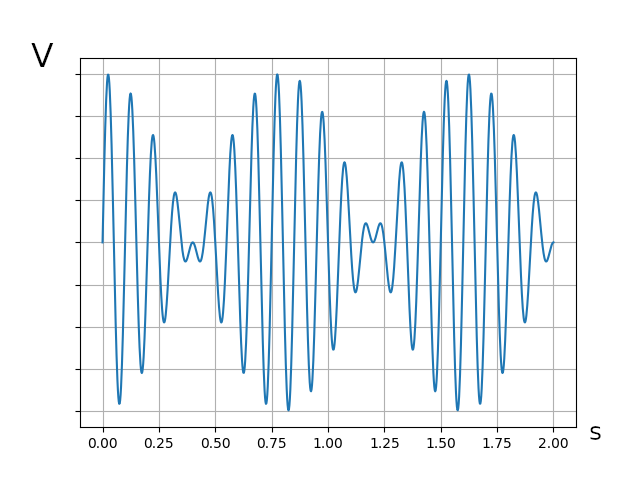
\includegraphics[width=0.7\linewidth]{img/fig01}
\caption{Tracé de la réponse temporelle v(t)}
\label{fig01}
\end{figure}

Cette fonction est définie comme suit dans un script python qui va être complété:
\begin{center}
\begin{minted}[linenos,frame=lines]{python}
def theta(t):
    return 2*np.pi*fr*t

def v(t):
    return Vr*np.sin(k*theta(t))*np.cos(theta(t))

t=np.linspace(0,2,1000)
plt.plot(t,v(t))
\end{minted}
\end{center}

\subsection{Recherche de $V_{r\ max}$}

On propose deux scripts pour compléter le précédent afin de déterminer la valeur de $V_{r\ max}$.

~\

\begin{minipage}{0.45\linewidth}
\begin{center}
Solution A
\begin{minted}[linenos,frame=lines]{python}
m=v(t[i])
while v(t[i])<=m:
    if v(t[i])>m:
        m=v(t[i])
print(m)
\end{minted}
\end{center}
\end{minipage}\hfill
\begin{minipage}{0.45\linewidth}
\begin{center}
Solution B
\begin{minted}[linenos,frame=lines]{python}
m=v(0)
for ti in t:
    if v(ti)>m:
        m=v(ti)        
print(m)
\end{minted}
\end{center}
\end{minipage}

\question{Choisir en justifiant la solution qui permet de déterminer $V_{r\ max}$.}

Le résultat affiché par le script qui convient est \verb?9.9519?.

\question{En déduire en justifiant la valeur de $V_{r\ max}$.}

\subsection{Identification de $k$}

On montre que la courbe de la figure \ref{fig01}, coupe $2\cdot k$ fois la droite d'équation $y=1$ sur l'intervalle $\left[0,\frac{1}{f_r}\right]$. L'objectif de la suite est de déterminer le nombre d'intersections afin d'en déduire $k$.

\paragraph{Recherche des intervalles $[t,t+dt]$, incluant un passage par y=1} ~\ \\

On souhaite dans cette partie créer une liste \verb?bornes?, contenant l'ensemble des intervalles $[t,t+dt]$ tels qu'il existe un $t_p\in[t,t+dt]$ tel que $v(t_p)=1$.

Une fois la liste créée, en tapant \verb?print(bornes[0:last])?, on obtient le résultat suivant:
\verb?[[0.0, 0.002002002002002002], [0.050050050050050046, 0.05205205205205205],?\\
\verb?[0.1041041041041041, 0.1061061061061061], [0.15415415415415415, 0.15615615615615616]]?

Cela signifie que la courbe $v(t)$ coupe $y=1$ entre $0$ et $0.002002002002002002$, etc...

\question{Quelle valeur de \verb?last? permet l'affichage précédent ?}

\question{Écrire un script python permettant de détecter puis d'écrire dans la liste \verb?bornes? l'ensemble des intervalles définis précédemment.}

\paragraph{Recherche des solutions par dichotomie} ~\ \\

Voici le principe de la dichotomie:
\begin{itemize}
 \item Au rang 0,
 \begin{itemize}
  \item soient $a_0=a$, $b_0=b$. Il existe une solution $x_0$ de l'équation $(f(x)=0)$ dans l'intervalle $[a_0,b_0]$.
 \end{itemize}
 \item Au rang 1,
 \begin{itemize}
  \item si $f(a_0).f(\dfrac{a_0+b_0}{2})\leq 0$, alors on pose $a_1=a_0$, $b_1=\dfrac{a_0+b_0}{2}$,
  \item sinon on pose $a_{1}=\dfrac{a_0+b_0}{2}$ et $b_1=b$.
  \item dans les deux cas, il existe une solution $x_1$ de l'équation $(f(x)=0)$ dans l'intervalle $[a_1,b_1]$.
 \end{itemize}
 \item Au rang n, supposons construit un intervalle $[a_n,b_n]$, de longueur $\dfrac{b-a}{2^n}$,  et contenant une solution $x_n$ de l'équation $(f(x)=0)$. Alors:
 \begin{itemize}
  \item  si $f(a_n).f(\dfrac{a_n+b_n}{2})\leq 0$, alors on pose $a_{n+1}=a_n$, $b_{n+1}=\dfrac{a_n+b_n}{2}$,
  \item sinon on pose $a_{n+1}=\dfrac{a_n+b_n}{2}$ et $b_{n+1}=b_{n}$,
  \item dans les deux cas, il existe une solution $x_{n+1}$ de l'équation $(f(x)=0)$ dans l'intervalle $[a_{n+1},b_{n+1}]$.
 \end{itemize}
\end{itemize}

~\

À chaque étape, on a $a_n\leq x_n \leq b_n$, on arrête le processus dès que $|f(\frac{a_n+b_n}{2})|$ est inférieure à la précision souhaitée.

\question{Écrire un script python permettant de rechercher par dichotomie la solution de l'équation \verb?f(x)=0? entre \verb?a? et \verb?b? avec une précision \verb?p?.}

\question{Créer une fonction \verb?dichotomie(f,a,b,p)? à partir de ce script. (si vous n'avez pas réussi la question précédente, créer une fonction qui permet de calculer $f(a+b+p)$.}

~\

Le script suivant utilise la fonction \verb?dichotomie(f,a,b,p)? précédente.

\begin{center}
\begin{minted}[linenos,frame=lines]{python}
def g(t):
    return v(t)-1

p=10**(-6)
l1=[]
l2=[]
for borne in bornes:
    x=dichotomie(g,borne[0],borne[1],p)
    if x<1/fr:
        l1.append(x)
        l2.append(v(x))
\end{minted}
\end{center}

\question{Expliquer l'intérêt de la fonction \verb?g(t)?.}

\question{Expliquer à quels types de variables appartiennent \verb?l1? et \verb?l2? et ce qu'elles contiennent.}

\question{Expliquer l'intérêt du test \verb?if x<1/fr? dans ce script.}

~\

La fonction \verb?len(list)? renvoie le nombre d'éléments de la liste \verb?list?.

\question{Proposer une solution pour déterminer $k$.}

\section{Valeur approchée de $\xi$}

On souhaite modifier la valeur de $f_r$ et choisir maintenant $f_r=0,7~\textrm{Hz}$.

\question{Écrire sous la forme d'un mot de 32 bits respectant la norme IEEE 754 (signe, exposant, mantisse) le float $0,7$.}

\question{Montrer que $001100110011001100110011_2=\frac{2^{24}-1}{5}.$}

~\

On donne: $\frac{2^{-24}}{5}\approx 1.2*10^{-8}$.

\question{Déterminer l'erreur due au stockage de 0,7 à l'aide de la norme IEE74.}

\newpage

\section{Document réponse}

Nom:.....................\\
Prénom:......................

\begin{center}
 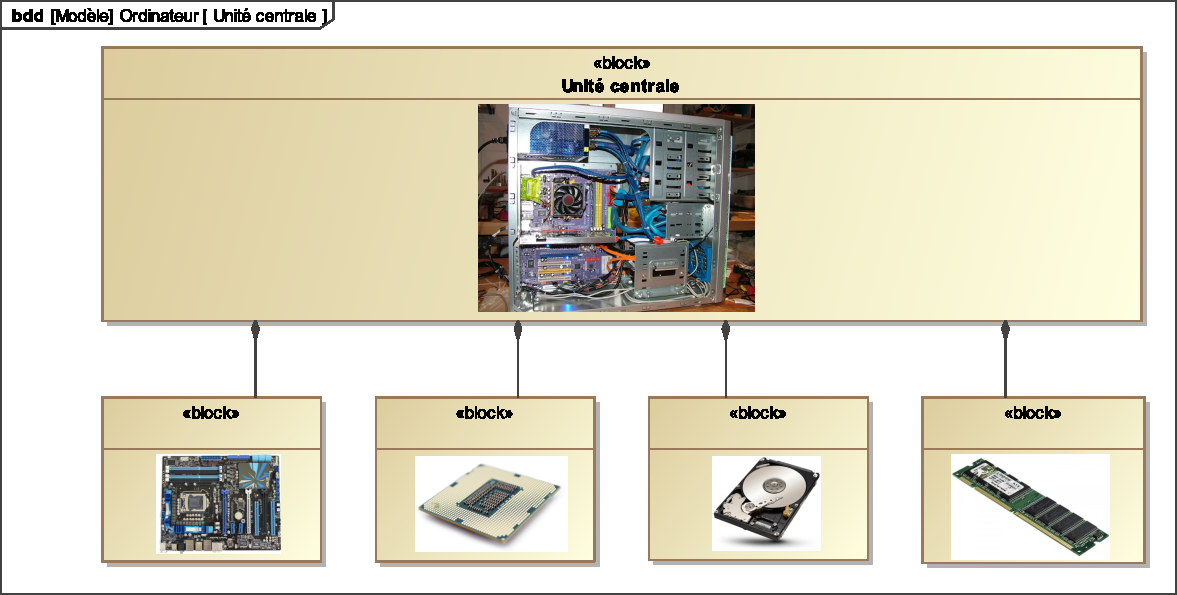
\includegraphics[width=0.9\linewidth]{img/unite_centrale_vierge}
\end{center}

\ifdef{\public}{\end{document}}{}

\newpage

~\

\newpage
\cleardoublepage

\pagestyle{correction}\setcounter{section}{0}

\section{Correction}

\paragraph{Question 1:}

\begin{center}
 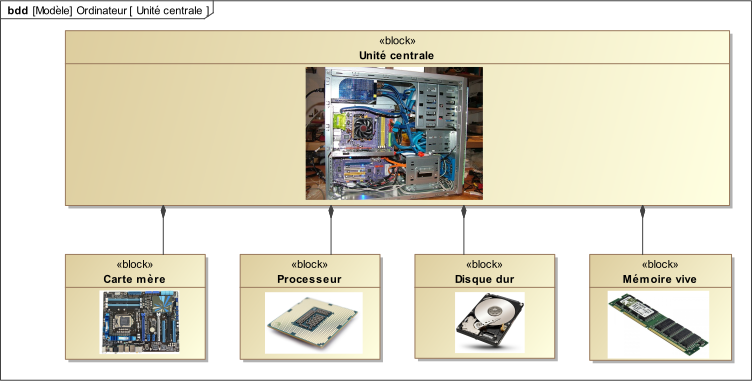
\includegraphics[width=0.9\linewidth]{img/unite_centrale_corrige}
\end{center}

\paragraph{Question 2:}

La solution à choisir est la B, la A ne fonctionne pas dès la première ligne car \verb?i? n'est pas défini. De plus, il faut ici parcourir toute la liste pour chercher un maximum, il faut donc une boucle \verb?for? et non \verb?while?.

\paragraph{Question 3:}

La valeur de $V_{\ max}$ est un entier, vu la valeur obtenue on suppose que le premier entier supérieur doit être la bonne réponse, donc $V_{\ max}=10~\textrm{V}$.

\paragraph{Question 4:}

Il y a 4 éléments dans la liste, ce sont donc les 0, 1, 2 et 3ème, donc \verb?last=4?.

\paragraph{Question 5:}

\begin{center}
\begin{minted}[frame=lines]{python}
bornes=[]
for i in range(1,len(t)):
#    if v(t[i-1])>1 and v(t[i])<1 or v(t[i-1])<1 and v(t[i])>1: (autre solution)
    if (v(t[i-1])-1.)*(v(t[i])-1.) < 0:
        bornes.append([t[i-1],t[i]])
\end{minted}
\end{center}

\paragraph{Question 6:}

\begin{center}
\begin{minted}[frame=lines]{python}
m=(a+b)/2.
while np.abs(v(m)) >  p:
    m=(b+a)/2.
    if v(a)*v(m) > 0:
        a=m
    else:
        b=m
\end{minted}
\end{center}

\paragraph{Question 7:}


\begin{center}
\begin{minted}[frame=lines]{python}
def dichotomie(f,a,b,p):
    m=(a+b)/2.
    while np.abs(f(m)) >  p:
        m=(b+a)/2.
        if f(a)*f(m) > 0:
            a=m
        else:
            b=m
    return m
\end{minted}
\end{center}

Si pas de question 6

\begin{center}
\begin{minted}[frame=lines]{python}
def dichotomie(f,a,b,p):
    return f(a+b+p)
\end{minted}
\end{center}

\paragraph{Question 8:}

La fonction $g(t)=v(t)-1$ permet de rechercher la solution $v(t)=1$ et non pas $v(t)=0$.

\paragraph{Question 9:}

\verb?l1? et \verb?l2? sont des listes qui contiennent:
\begin{itemize}
 \item \verb?l1?: la liste des instants $t$ où $v(t)=1$ (abscisses),
 \item \verb?l2?: la liste des $v(t)$ à ces instants là (ce sont des valeurs proches de 1) (ordonnées).
\end{itemize}

\paragraph{Question 10:}

Ce test permet de ne prendre en compte que les solutions dans l'intervalle $\left[0,\frac{1}{f_r}\right]$ comme demandé dans l'énoncé.

\paragraph{Question 11:}

La courbe passe 2 fois par $1$ à chaque période, on a donc \verb?k=len(l1)/2.?

\paragraph{Question 12:}

Le nombre à traduire est $0,7_{10}$.

\begin{tabular}{c c c c c c c c c c}
0,7 & x & 2 & = & 1,4 & = &  1 & + & 0,4 \\
0,4 & x & 2 & = & 0,8 & = &  0 & + & 0,8 \\
0,8 & x & 2 & = & 1,6 & = &  1 & + & 0,6 \\
0,6 & x & 2 & = & 1,2 & = &  1 & + & 0,2 \\
0,2 & x & 2 & = & 0,4 & = &  0 & + & 0,4 \\
0,4 & x & 2 & = & 0,8 & = &  0 & + & 0,8 \\
0,8 & x & 2 & = & 1,6 & = &  1 & + & 0,6 \\
...
\end{tabular}

On remarque un récurrence dans l'écriture du $0,7_{10}$ en binaire: $0,7_{10}=0,1011001100.._2$

Le nombre stocké est alors :
$1,\underbrace{01100110011001100110011_2}_{23 bits}*2^{-1}$

\begin{itemize}
 \item Signe = $0$,
 \item Mantisse:$\underbrace{01100110011001100110011_2}_{23 bits}$,
 \item Exposant:$127-1=126_{10}=01111110_2$
\end{itemize}

\paragraph{Question 13:} ~\ \\

$a=\underbrace{001100110011001100110011}_{24 bits}=\underbrace{111111111111111111111111}_{24 bits}-
\underbrace{110011001100110011001100}_{24 bits}=
(2^{24}-1)-4*a$, donc $a=\frac{2^{24}-1}{5}$.

\paragraph{Question 14:}

Le nombre stocké est donc: $101100110011001100110011.2^{-24}=(2^{23}+\frac{2^{24}-1}{5}).2^{-24}=(\frac{1}{2}+\frac{1}{5}-\frac{2^{-24}}{5})$.

L'erreur est donc de $-\frac{2^{-24}}{5}=-1.2*10^{-8}$

\end{document}
